\section{Detector Performance}
\label{sec:performance}

Data at different beam energies and with different trigger conditions have been analyzed to study and assess the
FT performance. Results from the studies are detailed below.

\subsection{Acceptance}

The detector acceptance was studied in detail at the maximum beam energy the experiment operated at so far of
10.6~GeV. Data were recorded with a minimum-bias trigger based on the FT-Cal alone with a threshold on the
measured cluster energy of 100~MeV. In the offline analysis, events were further selected, requiring a reconstructed
electron via the matching of the FT-Cal cluster to FT-Hodo hits, and the associated FT-Cal cluster to have total energy
greater than 500~MeV, seed energy greater than 300~MeV, and size greater than or equal to 4 crystals. The resulting
event distributions as a function of the electron energy and polar angle are shown in Fig.~\ref{fig:ft_acceptance}. 

The energy coverage extends from 500~MeV, as selected in the offline analysis, up to the end-point, set by the
beam energy, where elastic scattering dominates. Close to the energy end-point, the detector resolution is expected
to worsen significantly because of saturation of the FT-Cal preamplifiers and FADCs that are optimized for the
design energy range of 0.5-4.5~GeV. The $\theta$ range extends from the minimum angle of 2.5$^\circ$ to
$\sim$5$^\circ$. The two-dimensional distribution shows the effect of the CLAS12 solenoid field on low-momentum
electrons starting from $\theta\sim2^\circ$ that are bent into the detector acceptance. The detector
acceptance matches and partially exceeds the design specifications. 

\begin{figure}[ht]
\begin{center}
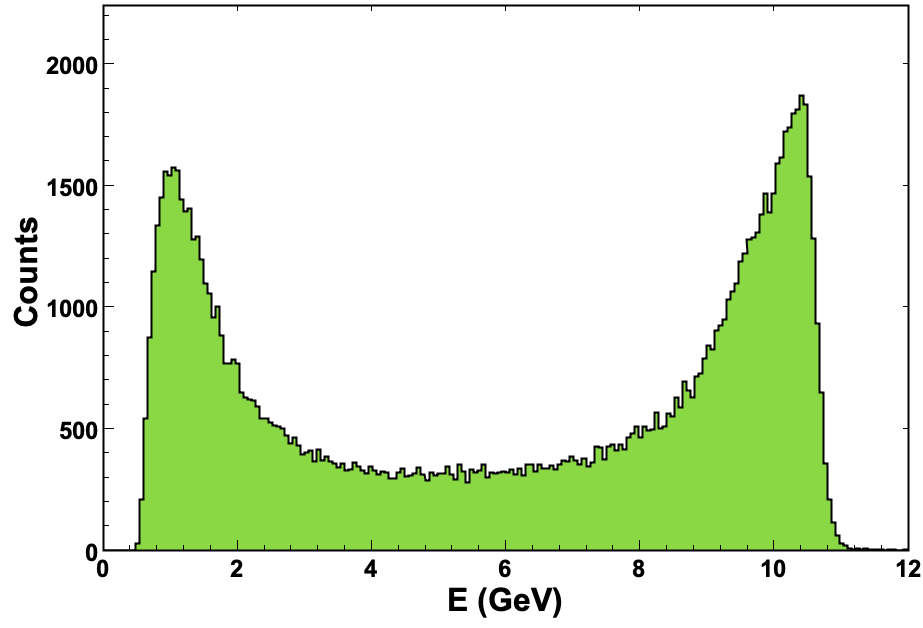
\includegraphics[height=0.5\columnwidth]{fig/ft_acceptance_energy.png}
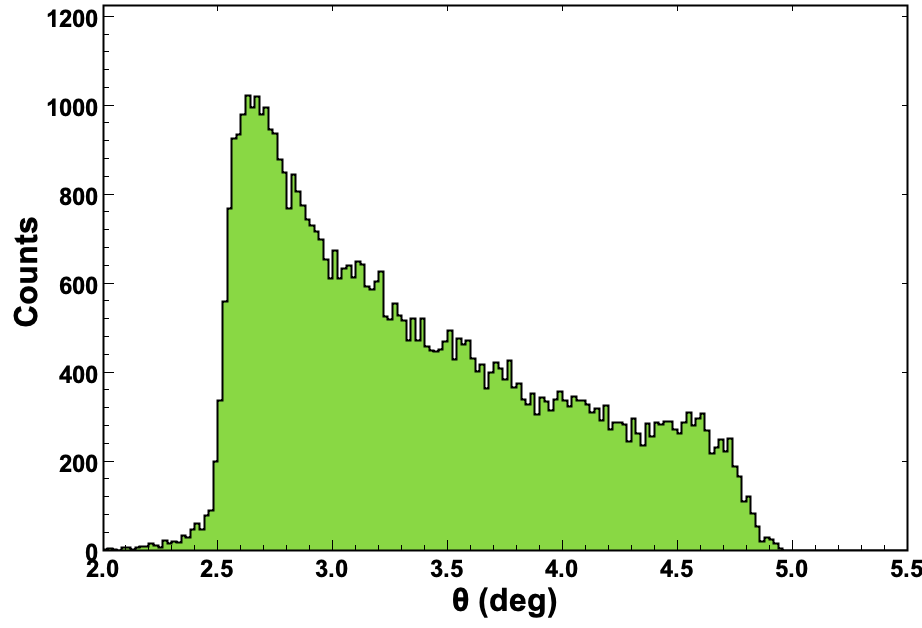
\includegraphics[height=0.5\columnwidth]{fig/ft_acceptance_theta.png}
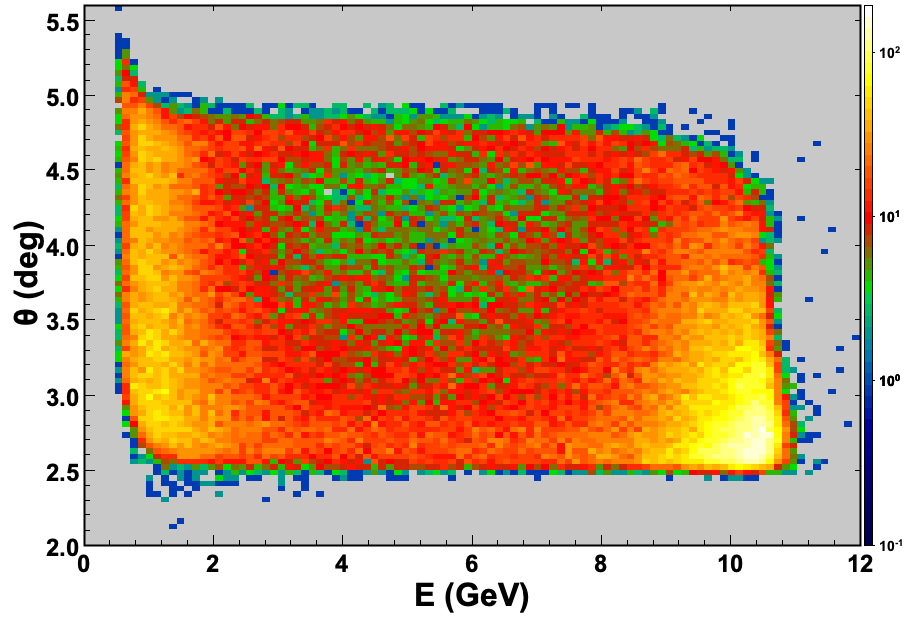
\includegraphics[height=0.5\columnwidth]{fig/ft_acceptance_energytheta.png}
\end{center}
\caption{FT acceptance for electrons as a function of energy (top), polar angle (middle), and of both
  variables (bottom) at 10.6~GeV beam energy. The energy range goes from 500~MeV, as selected in the offline
  analysis, up to the end-point set by the beam energy where elastic scattering dominates. The $\theta$ range goes
  from the minimum angle of 2.5$^\circ$ to $\sim$5$^\circ$. The two-dimensional distribution shows the effect of the
  CLAS12 solenoid field on low-momentum electrons that start from $\theta\sim2^\circ$ and are bent into the
  detector acceptance. }
\label{fig:ft_acceptance}
\end{figure}

\begin{figure}[h]
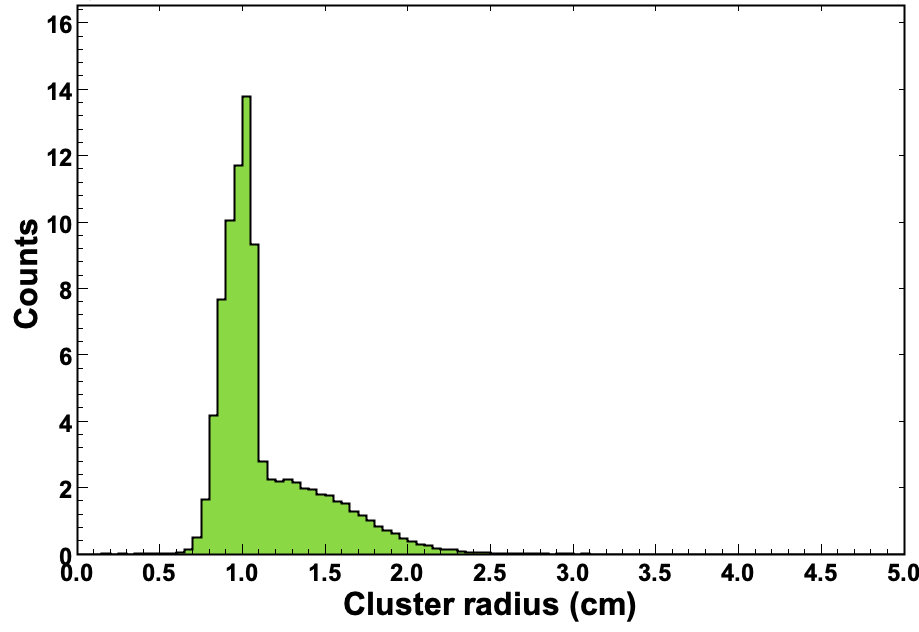
\includegraphics[height=0.65\columnwidth]{fig/ft_shower.png}
\caption{Radius of the FT-Cal shower for charged particles. A clear peak at $\sim$1~cm associated with
  electron-induced electromagnetic showers overlaps with a broader distribution due to hadronic showers.}
\label{fig:ft_shower}
\end{figure}

\subsection{Energy Resolution and Electromagnetic Shower Reconstruction}

Within the detector acceptance, the energy resolution was studied based on elastic scattering and $\pi^0$ decay to
two photons, as discussed in Section.~\ref{sec:calibration}. The results indicate the currently achieved resolution is
larger than the design value by about 1\% at 2~GeV. The reasons for this discrepancy can be multi-fold. First, the
energy calibration of individual crystals has shown a significant spread in the energy-to-charge conversion that was
not foreseen in the initial estimates. This spread, likely due to the non-uniformity of the crystal light yield, can
contribute to a worsening of the resolution because it results in a non-homogeneous detector response.  Second, as a consequence of the crystal non-uniformity, the threshold applied in the cluster reconstruction is for some crystals larger than the 10 MeV used in the simulation studies and prototype analyses.

The shower profile in the FT-Cal was studied and compared to Monte Carlo simulations for different particle
species. Figure~\ref{fig:ft_shower} shows the shower radius, defined as the square root of the second moment of
the shower, for charged particles, i.e. particles associated to a cluster in the calorimeter with matching hits in the
hodoscope. A clear peak with radius of $\sim$1~cm associated with electrons is clearly visible, overlapping a
broader distribution associated with hadronic showers. The shower profile and, specifically the cluster radius, can
therefore be used to discriminate between different particle types.

\begin{figure}[h]
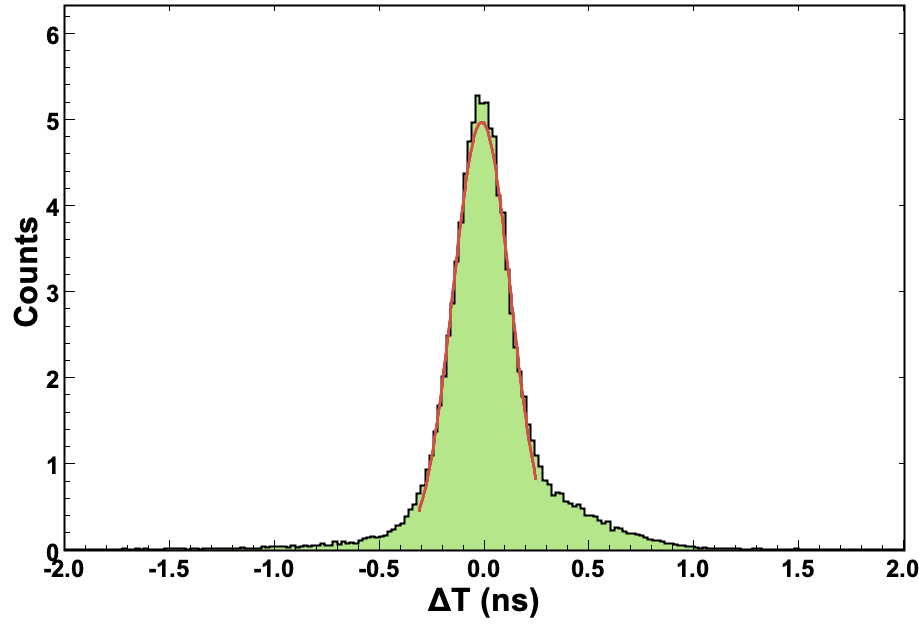
\includegraphics[height=0.6\columnwidth]{fig/ft_electron_time.png}
\caption{Time resolution for electrons detected in the FT with energy greater than 500~MeV, seed
  energy greater than 300~MeV, and cluster size larger or equal to 4. The histogram shows the time difference
  between the FT time projected back to the event vertex and the RF signal time. The Gaussian fit gives a resolution
  $\sigma \sim$140~ps.}
\label{fig:electron_time}
\end{figure}

\subsection{Timing Resolution}

\begin{figure}[h]
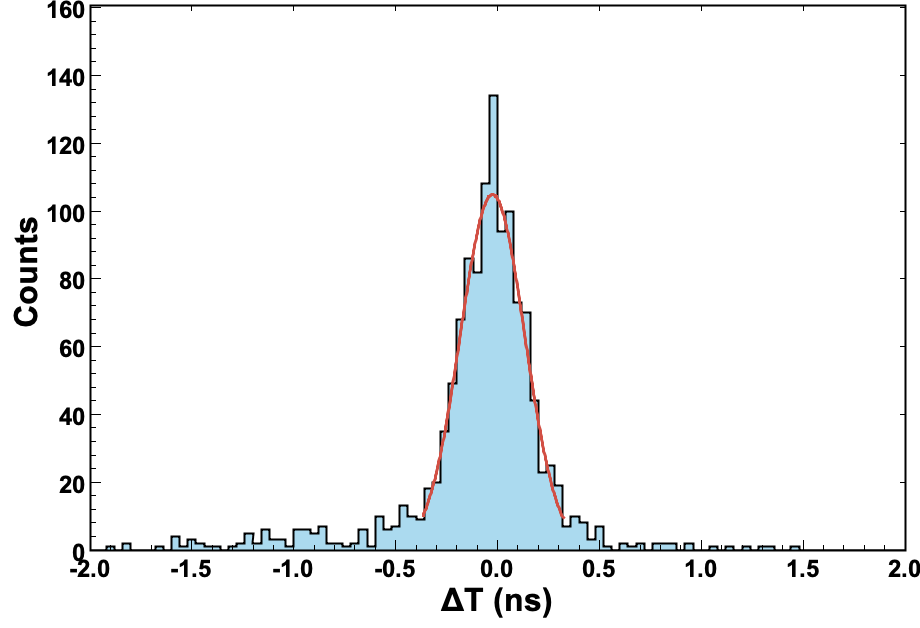
\includegraphics[height=0.6\columnwidth]{fig/ft_gamma_time.png}
\caption{Time resolution for photons detected in the FT with energy greater than 500~MeV, seed
  energy greater than 300~MeV, and cluster size greater or equal to 4. The histogram shows the time difference
  between the FT time projected back to the event vertex and the event start time derived from the CLAS12 FTOF
  detector for events where an electron is identified in the CLAS12 Forward Detector. The Gaussian fit gives a
  resolution $\sigma \sim$150~ps. }
\label{fig:gamma_time}
\end{figure}

The timing resolution for electrons and photons was evaluated from beam data by correlating the reconstructed
cluster time from the FT-Cal to either the RF signal that is synchronous with the CEBAF accelerator beam bunches
or the event start time derived from the CLAS12 Forward Time-of-Flight (FTOF) system~\cite{ftof}.
Specifically, the electron time resolution was studied correlating the FT time projected back to the event vertex
to the RF signal time. The difference of these two times for 10.6~GeV data is shown in Fig.~\ref{fig:electron_time}
for electrons with energy greater than 500~MeV, cluster seed energy greater than 300~MeV, and cluster size
greater than or equal to 4 crystals: a Gaussian fit to the distribution gives $\sigma \sim$140~ps. The tails of the
distribution are due to low-energy clusters close to the applied selection threshold, and are expected to be reduced
by improvements of the time-walk correction that are currently under study.

While this estimate of the resolution relies solely on the FT reconstruction, an alternative measure can be
performed by selecting photons detected in the FT and correlating their time to the event start time determined
from other particles detected in CLAS12. This analysis was performed for events with an electron detected in
the CLAS12 Forward Detector whose start time is determined based on the FTOF system and a photon detected in
the FT with energy greater than 500~MeV, cluster seed energy greater than 300~MeV, and cluster size greater than
or equal to 4 crystals. The photon FT time projected back to the event vertex was correlated with the event start time as
shown in Fig.~\ref{fig:gamma_time}. A Gaussian fit to the distribution gives $\sigma \sim$150~ps, slightly
larger but consistent with the electron timing resolution.

\begin{figure}[h]
  \centering
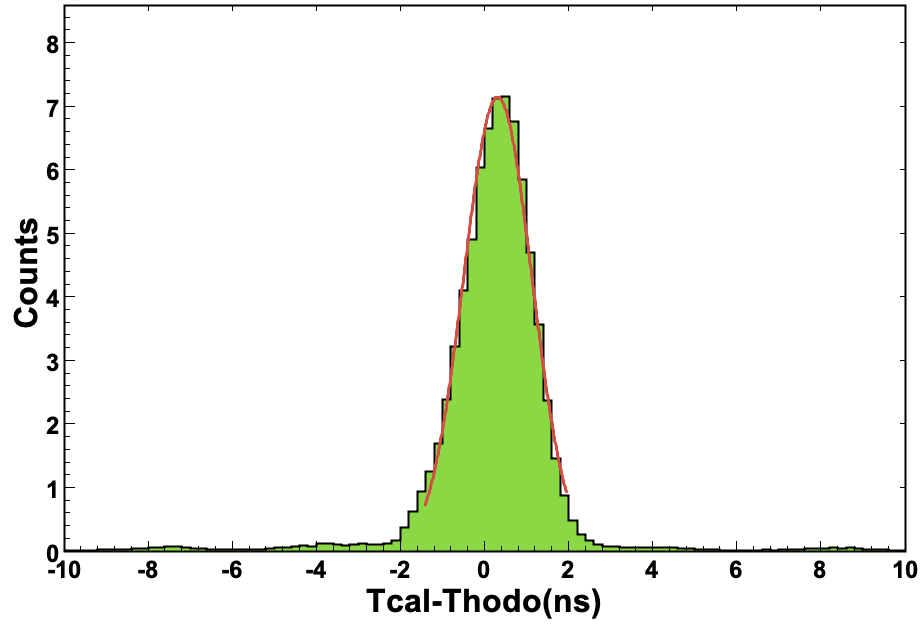
\includegraphics[height=0.6\columnwidth]{fig/ftcalhodo_time.png}
\caption{Time difference between the calorimeter and hodoscope clusters for reconstructed electrons: a Gaussian fit
  to the distribution gives $\sigma \sim$0.8~ns.}
\label{fig:ftcalhodo_time}
\end{figure}

While the FT time is determined by the calorimeter since this is the component with the best timing resolution,
the time correlation between the FT detectors is important to match the signals detected in the three
sub-components and minimize accidentals. Figure~\ref{fig:ftcalhodo_time} shows the time difference of the
reconstructed calorimeter and hodoscope clusters for detected electrons with $\sigma \sim$0.8~ns,
dominated by the hodoscope resolution. The value is consistent with the design resolution for the hodoscope of
$<$1~ns.

\subsection{Trigger Performance}

The FT is used as an active component of the CLAS12 trigger system to identify events in which electrons or
photons are detected in the system. This is achieved by reconstructing in real time clusters in the calorimeter with
or without geometrical and time matching with hodoscope tiles. Details on the trigger algorithms, their implementation,
and validation are provided in Ref.~\cite{trigger}, while here we focus only on reporting the performance in terms of
linearity of the trigger rate as a function of luminosity. This was studied performing a luminosity scan and recording
the FT trigger rate at the input of the data acquisition system. Figure~\ref{fig:trigger_rate} shows the measured
dependence. These results confirm the linearity of the FT trigger up to the maximum luminosity foreseen for the
experiment.

\begin{figure}[h]
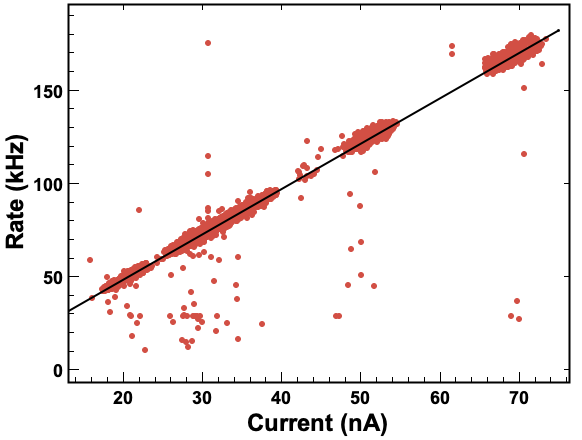
\includegraphics[height=0.68\columnwidth]{fig/ft_trigger.png}
\caption{FT trigger rate as a function of the beam current. The measurements are consistent with a linear dependence
  up to the maximum CLAS12 luminosity of $10^{35}$~cm$^{-2}$s$^{-1}$, which is obtained at a current of 75~nA on a
  5-cm-long liquid-hydrogen target. The points that deviate from the linear slope correspond to measurements with
  unstable beam conditions.}
\label{fig:trigger_rate}
\end{figure}

